\documentclass[a4paper,12pt,oneside,onecolumn,openany,final]{memoir}

% Preamble
%-----------------------------------------------------------------------------------------
\usepackage{thesis_preamble}

\title{Applications of Galois Theory}
\author{Sandesh Thakuri}

%------------------------------------------------------------------------------------------

\begin{document}

\frontmatter
% --------------------------------------------------------------------------------------------

\maketitle
\clearpage

\maxtocdepth{subsection} % put 3 levels into the ToC
\tableofcontents  %table of contents

\mainmatter
% ---------------------------------------------------------------------------------------------

\addcontentsline{toc}{chapter}{Symbol Conventions Used}

{\LARGE {\textbf{Symbol Conventions}}}

  \vspace{9mm}

Through out the thesis following Symbol Convention has been used.\\[4mm]

\begin{itemize}
\item \textbf{K} \hspace{5mm} a field.
\item \textbf{F} \hspace{5mm} an extension field of the field \textbf{K}
\end{itemize}


\part{Galois Theory}

\chapter{Field Extension}
\begin{wrapfigure}{r}{0.3\textwidth}
  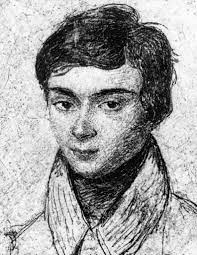
\includegraphics[width=45mm, height=57mm]{galois.jpg}
  \caption{\footnotesize Portrait of Galois}
\end{wrapfigure}

Galois Theory is a popular and one of the important theory in Abstract Algebra. It's foundation was laid by the French Mathematician \textit{Évariste Galois} by determining the necessary and sufficient condition for solving a polynomial equation by radicals and thereby solving the problem that was open for 350 years old \cite{galois}.\\ \\
The core-part of the Galois Theory is the \textit{Fundamental Theorem} of Galois Theory which links two main parts of Abstract Algebra; Field Theory and Group Theory. This is a profound result in Abstract Algebra.

\vspace{15mm}
\section{Approaches to the Theory}
\begin{enumerate}
\item Galois approached this problem by using the group of permutations of the roots of a polynomial equation. Only those permutations of the roots are considered which leaves any equation satisfied by the roots unchanged.

\item The modern approach is to use the \textbf{field extension} of the underlying field of the polynomial and examine the groups of automorphism of the extension field that fixes the underlying field.
\end{enumerate}
So, the Galois theory is the theory of field extensions.
\clearpage

\section{Structure of a Field Extension}
Let \(F=K(u)\) be a field extension of the field \(K\). Then \(F\) is a vector space over \(K\) generated by \(u\).\\
We have \(u^n \in F\) for all \(n \in \mathbb{Z}\) because F is a field. As \(F\) is a vector space over \(K\); \(F\) consists of all linear combinations of \(u^n \)'s, and the quotients of these linear combinations. A such linear combinations is: \(a_nu^n+a_{n-1}u^{n-1}+...+a_1u+a_0\) which is  given by the polynomial \(f(u)\), where \(f(x)=a_nx^n+a_{n-1}x^{n-1}+...+a_1x+a_0\).\\

So the structure of the extension field \(F=K(u)\) is:\\
\(F= \{\frac{f(u)}{g(u)} \;| \; f,g \in K[x],g(u) \neq 0\}\).\\

\begin{theorem}[Existence of an Extension field]
If K is a field and \(f \in K[x]\) is a polynomial of degree \(n\),then there exists a simple extension field \(F=K(u)\) of K such that \(u\in F\) is a root of \(f\)\cite{hunger}.
\end{theorem}

\section{Algebraic and Transcendental element}
\begin{theorem}
Let \(F\) be an extension field of a field \(F\).\\
A map \(\phi:K[X] \rightarrow K[u]\) where \(u \in F\) defined by \(\phi (f(x))=f(u)\)\\
i.e, \(\phi (a_0+a_1x+...+a_nx^n)= a_0+a_1u+...+a_nu^n\) is a ring homomorphism \cite{hunger}.
\end{theorem}

Thus \( K[x]\) and \(K[u]\) are homomorphic.
  \begin{enumerate}
  \item If \(u\) is transcendental over \(K\) then \(K[u]\) is not a field and \(K[x] \cong K[u]\).
  \item If \(u\) is algebraic over \(K\) then, \(K[x] \ncong K[u]\) because \(Ker\phi\) is non trival and we have,
    \begin{enumerate}
    \item[i)] \(K(u) \cong K[u]\);
    \item[ii)] \(K(u) \cong K[x]/(f)\), where \(f \in K[x]\) is an irreducible monic polynomial of degree \(n \geq 1\);
    \item[iii)] \([K(u):K]=n\) and \(\{1_k,u,u^2,...,u^{n-1}\}\) is a basis of the vector space \(K(u)\) over \(K\).
    \end{enumerate}
  \end{enumerate}

\begin{theorem}[Isomorphism of Extension fields]
 Let K be a field.\\
 Then 'u' and 'v' are  roots of the same irreducible polynomial \(f \in K[x]\) if and only if there is an isomorphism of fields \(K[u] \cong K[v]\) which sends u onto v and is the identity on \(K\) \cite{hunger}.
\end{theorem}



%%% Local Variables:
%%% mode: latex
%%% TeX-master: "n"
%%% End:


\chapter{Galois Theory}
``Galois extension \(F\) of  \(K\) is a field for which the fixed field of the Galois group \(Aut_K^F\) is \(K\) itself'' \cite{hunger}.\\
But for what extension field \(F\) of \(K\) the Galois group keeps the ``base field \(K\)'' fixed? What is the structure of Galois field and how do we construct(obtain) a Galois field?


\section{Splitting Field}
Since, for \(F=K(u)\), any \(\sigma \in Aut_K^F\) is ``completely determined'' \cite{hunger} by its action on \(u\). Any algebraic Galois extension of \(K\) is generated by all roots \(u\) of a polynomial \(f \in K[x]\) \cite{hunger}.

\begin{definition}
  Such a minimal field \(F\) where a polynomial \(f \in K[x]\) ``splits into linear factors'' and thus ``contains all roots of \(f(x)\)'' is called a splitting field of \(f\) over \(K\) \cite{hunger}.
\end{definition}
Thus, an algebraic Galois extension is going to be characterized by ``a splitting field of a polynomial over the base field'' \cite{hunger}.\\

\begin{theorem}[Existence of a Splitting field]
  ``If \(K\) is a field and \(f \in K[x]\) has degree \(n \geq 1\), then there exists a splitting field \(F\) of \(f\) with \([F:K] \leq n!\)'' \cite{hunger}.
  \end{theorem}

\subsection{Algebraic Closure of a Field}
``A field \(F\) is said to be algebraically closed if every nonconstant polynomial \(f \in F[x]\) has a root in \(F\)'' \cite{hunger}.
For example the field of complex number \(\mathbb{C}\) is algebraically closed.\\ \\

\begin{definition}
An extension field \(F\) of a field \(K\) is said to be algebraic closure of \(K\) if,
\begin{enumerate}
\item[i)] F is algebraically closed and,
  \item[ii)] F is algebraic over \(K\) \cite{hunger}.
  \end{enumerate}
\end{definition}


So, \(\mathbb{C}\) is algebraically closed field but is not an algebraic closure of \(\mathbb{Q}\) because \(\mathbb{C}\) is not algebraic over \(\mathbb{Q}\) \cite{hunger}.
But \(\mathbb{C}\) is an algebraic closure of \(\mathbb{R}\).\\
This shows algebraic closure is an special case of a splitting field.

\section{Separable Extension}
``An irreducible polynomial \(f \in K[x]\) is said to be separable if in some splitting field of \(f\) over \(K\) every root of \(f\) is a simple root'' \cite{hunger}.\\
An algebraic element \(u \in F\) is said to be ``separable over \(K\) provided its irreducible polynomial is separable''\cite{hunger}.
\begin{definition}
  ``If every element of \(F\) is separable over \(K\), then \(F\) is said to be a separable extension of \(K\)'' \cite{hunger}.\\[3mm]
\end{definition}
\noindent
\textbf{Characteristic of a Separable extension}
\begin{remark}
  ``Every algebraic extension field of a field of characteristic \(0\) is separable'' \cite{hunger}.
  \end{remark}
If a polynomial \(f \in K[x]\) is separable over \(K\) then it has no multiple roots in any splitting field of \(f\) over \(K\) \cite{hunger}. ``This shows that an irreducible polynomial in \(K[x]\) is separable if and only if its derivative is nonzero'' \cite{hunger}. This holds true for every field of characteristic zero \cite{hunger}.

\section{Galois extension}
\begin{theorem}
  ``\(F\) is algebraic and Galois over \(K\) if and only if \(F\) is separable over \(K\) and \(F\) is a splitting field over \(K\) of a set \(S\) of polynomials in \(K[x]\)'' \cite{hunger}.\\
  \end{theorem}

This proves the \textbf{Generalized Fundamental Theorem of Galois Theory},\\
which sates the \textit{Fundamental Theorem of Galois Theory} still holds if the extension field \(F\) is not finite dimensional as-well i.e, if ``\(F\) is algebraic and Galois over \(K\)'' \cite{hunger}.


\chapter{Structure of Galois Extension}
\begin{definition}
  The Galois group of a polynomial \(f \in K[x]\) is the group \(Aut_K^F\), where \(F\) is a splitting field of \(f\) over \(K\) \cite{hunger}.
  \end{definition}

  \begin{theorem}
  Let \(G\) be a Galois group of a polynomial \(f \in K[x]\).
\begin{enumerate}
\item[i)] \(G\) is isomorphic to a subgroup of some symmetric group \(S_n\).
  \item[ii)] If \(f\) is separable of degree \(n\), the \(n\) divides \(|G|\) and \(G\) isomorphic to a transitive subgroup of \(S_n\) \cite{hunger}.
  \end{enumerate}
\end{theorem}
Because the Galois group \(Aut_K^F\) is a group of automorphisms of F which is given by the permutations of the roots.
So, the Galois group of a polynomial is identified with the subgroup of \(S_n\).\\

\begin{corollary}
\begin{enumerate}
\item[i)] If the degree of \(f\) is \(2\) then its Galois group \(G \cong {\mathbb{Z}}_2\).
  \item[ii)] If the degree of \(f\) is \(3\) then its Galois group \(G\) is either \(S_3\) or \(A_3\) \cite{hunger}.
  \end{enumerate}
\end{corollary}


\section{Galois Group of Cubic polynomials}
\begin{definition}
  Let \(K\) be a field with \(char K \neq 2\) and \(f \in K[x]\) a polynomial of degree \(n\) with \(n\) distinct roots \(u_1,u_2,...,u_n\) in some splitting field \(F\) of \(f\) over \(K\). Let \(\Delta = \prod\limits_{i<j}(u_i-u_j) = (u_1-u_2)(u_1-u_3)...(u_{n-1}-u_n) \in F\).\\
  The discriminant of \(f\) is the element \(D= {\Delta}^2\) \cite{hunger}.
\end{definition}

\begin{theorem}
\begin{enumerate}
\item[i)] The discriminant \({\Delta}^2\) of \(f\) actually lies in \(K\).
  \item[ii)] For each \(\sigma \in Aut_K^F < S_n, \sigma\) is an even[resp. odd] if and only if \(\sigma(\Delta) = \Delta\)[resp. \(\sigma(\Delta) = - \Delta\)] \cite{hunger}.
  \end{enumerate}
\end{theorem}
Since \({\Delta}^2 \in K\) and \(\Delta \in F\), and \(K(\Delta)\) is a stable intermediate; in the Galois correspondence the subfield \(K(\Delta)\) corresponds to the subgroup \(G \cap A_n\). In particular, \(G\) consists of even permutations if and only if \(\Delta \in K\).

\begin{corollary}
  If \(f\) is a separable polynomial of degree \(3\), then the Galois group of \(f\) is \(A_3\) if and only if the discriminant of \(f\) is the square of an element of \(K\) \cite{hunger}.
\end{corollary}

\begin{theorem}
  Let \(K\) be a field of \(char K \neq 2,3 \). If \(f(x)=x^3+bx^2+cx+d \in K[x]\) has three distinct roots in some splitting field, then the polynomial \(g(x)=f(x-b/3) \in K[x]\) has the form \(x^3+p^2+q\) and the discriminant of \(f\) is \(-4p^3-27q^2\) \cite{hunger}.
\end{theorem}

\section{Galois Group of Quartic polynomials}
\begin{definition}[Resolvant Cubic of a Quartic]
Let \(K, f, F, u_i, V,\) and \(G=Aut_K^F<S_4\) be as in the preceding paragraph and \(\alpha=u_1u_2+u_3u_4,\) \(\beta=u_1u_3+u_2u_4,\) \(\gamma=u_1u_4+u_2u_3\).
The polynomial \( (x- \alpha)(x- \beta)(x- \gamma) \) is called the resolvant cubic of \(f\). The resolvant cubic is actually a polynomial over \(K\) \cite{hunger}.\\
\end{definition}
Now under the Galois correspondence the subfield \(K(\alpha, \beta, \gamma)\) corresponds to the normal subgroup \(V \cap G\) because \(K(\alpha,\beta,\gamma)\) is a splitting field of the resolvant cubic
whose Galois group is a subgroup of \(S_3\) and only normal subgroup of \(N\) of \(S_4\) with \(|N| \leq 6\) is \(V\), where \(V=\{(1),(12)(34),(13)(24),(14)(23)\}\).\\
Hence \(K(\alpha, \beta, \gamma)\) is Galois over \(K\) and \(Aut_K^{K(\alpha, \beta, \gamma)} = G/(G \cap V\).

\begin{remark} If \(K\) is a field and \(f = x^4+bx^3+cx^2+dx+e \in K[x]\), then the resolvant cubic of \(f\) is the polynomial \(x^3-cx^2+(bd-4e)x-b^2e+4ce-d^2 \in K[x]\) \cite{hunger}.\\ \\
\end{remark}

\begin{theorem}
  Let \(K\) be a field and \(f \in K[x]\) a separable quartic with Galois Group \(G\). Let \(\alpha, \beta, \gamma\) be the roots of the resolvant cubic of \(f\) and let \(m= [K(\alpha, \beta, \gamma) : K]\) then,
\begin{enumerate}
\item[i)] \(m=6 \Longleftrightarrow G=S_4\);
\item[ii)] \(m=3 \Longleftrightarrow G=A_4\);
\item[iii)] \(m=1 \Longleftrightarrow G=V\);
\item[iv)] \(m=2 \Longleftrightarrow G=D_4\) or \(G={\mathbb{Z}}_4\); in this case \(G={\mathbb{Z}}_4\) if \(f\) is irreducible over \(K(\alpha, \beta, \gamma)\) and \(G={\mathbb{Z}}_4\) otherwise \cite{hunger}.
  \end{enumerate}
\end{theorem}
This is because we have \([K(\alpha,\beta,\gamma):K] = |G/G \cap V|\).

\section{Galois Group of some Polynomials}

\begin{example}
The polynomial is \(f(x)=x^4-2 \in \mathbb{Q}[x]\).\\
This polynomial is irreducible and therefore separable over \(\mathbb{Q}\). The resolvant cubic is \(x^3+8x = x(x+2i\sqrt{2})(x-2i\sqrt{2})\) and
\(\mathbb{Q}(\alpha,\beta, \gamma)=\mathbb{Q}(i\sqrt{2})\) has dimension \(2\) over \(\mathbb{Q}\). \(x^4-2\) is irreducible over \(\mathbb{Q}(i\sqrt{2})\) because \(\sqrt[\leftroot{-3}\uproot{3}4]{2} \not\in \mathbb{Q}(i\sqrt{2})\).
Therefore the Galois group \(G \cong D_8\) \cite{hunger}.
\end{example}

Let \(F \subset \mathbb{C}\) be a splitting field over \(\mathbb{Q}\) of \(f(x)=x^4-2 \in \mathbb{Q}[x]\). If \(u\) is the positive real fourth root of 2, then the roots of \(f\) are \(u,\; -u,\; ui,\; -ui\). To find the  Galois group \(G = Aut_{\mathbb{Q}}^F\) of \(f\) which is a subgroup of \(S_4\), we find the permutations of the roots. To do so  we must choose an ordering of the roots, say \(u_1=u\), \(u_2=ui\), \(u_3=-u\), \(u_4= -ui\). The complex conjugation is an \(\mathbb{R}\)-automorphism of \(\mathbb{C}\) which clearly sends:\\
\(u \mapsto u\), \(-u \mapsto -u\), \(ui \mapsto -ui\) and \(-ui \mapsto ui\). \\
This induces a \(\mathbb{Q}\)-automorphism \(\tau\) of \(F=\mathbb{Q}(u,ui)\). As an element of \(S_4\), \(\tau=(24)\).
Now the generator of \(D_8\) containing \(\tau = (24)\) is \(\sigma = (1234)\). We have \(F=\mathbb{Q}(u,ui)=\mathbb{Q}(u,i)\),
so every \(\mathbb{Q}\)-automorphism of \(F\) is completely determined by its action on \(u\) and \(i\). Thus the elements of \(G\)
may be described either in terms of \(\sigma\) and \(\tau\) or by their action on \(u\) and \(i\). The information is summarized in the table:\\[1mm]
\begin{table}[h!]
\begin{tabular}{|c|c|c|c|c|c|c|c|c|}
  \hline
  \ & (1) & (24) & (1234) & (13)(24) & (1432) & (12)(34) & (13) & (14)(32) \\
  \ &  & \(\tau\)  & \(\sigma\) & \({\sigma}^2\) & \({\sigma}^3\) & \(\sigma \tau\) & \({\sigma}^2 \tau\) & \({\sigma}^3 \tau\) \\
  \hline
  \(u \mapsto\) & \(u\) & \(u\) & \(ui\) & \(-u\) & \(-ui\) & \(ui\) & \(-u\) & \(-ui\) \\
  \(i \mapsto\) & \(i\) & \(-i\) & \(i\) & \(i\) & \(i\) & \(-i\) & \(-i\) & \(-i\) \\
  \hline
\end{tabular}
\caption{\footnotesize Roots permutation table.}
\end{table}

\vspace{4mm}
\begin{tikzpicture}

  \node[minimum width=3mm, minimum height=3mm, align=center] (i) {\((1)\)};

  \node[below of=i, minimum width=3mm, minimum height=3mm, align=center, yshift=-11mm] (ss) {\(<{\sigma}^2>\)};

  \node[left of=ss, minimum width=3mm, minimum height=3mm, align=center, xshift=-20mm] (sst) {\(<{\sigma}^2 \tau>\)};

  \node[
  left of=sst,
  minimum width=3mm,
  minimum height=3mm,
  align=center,
  xshift=-20mm
  ] (t) {\(<\tau>\)\>};

  \node[
  right of=ss,
  minimum width=3mm,
  minimum height=3mm,
  align=center,
  xshift=20mm
  ]
  (st) {\(<\sigma\tau>\)};

  \node[
  right of=st,
  minimum width=3mm,
  minimum height=3mm,
  align=center,
  xshift=20mm
  ]
  (ssst) {\(<{\sigma}^3\tau>\)};

  \node[
  below of=ss,
  minimum width=3mm,
  minimum height=3mm,
  align=center,
  yshift=-11mm
  ]
  (s) {\(<\sigma>\)};

  \node[
  left of=s,
  minimum width=3mm,
  minimum height=3mm,
  align=center,
  xshift=-30mm
  ]
  (iss) {\(<(1),{\sigma}^2,\sigma,\tau,{\sigma}^2\tau>\)};

  \node[
  right of=s,
  minimum width=3mm,
  minimum height=3mm,
  align=center,
  xshift=25mm
  ]
  (v) {\(V\)};

  \node[
  below of=s,
  minimum width=3mm,
  minimum height=3mm,
  align=center,
  yshift=-11mm
  ]
  (g) {\(G\)};

  \draw[{Stealth}-, thick] (i)--(t);
  \draw[{Stealth}-, thick] (i)--(sst);
  \draw[{Stealth}-, thick] (i)--(ss);
  \draw[{Stealth}-, thick] (i)--(st);
  \draw[{Stealth}-, thick] (i)--(ssst);

  \draw[{Stealth}-, thick] (ss)--(iss);
  \draw[{Stealth}-, thick] (ss)--(s);
  \draw[{Stealth}-, thick] (ss)--(v);

  \draw[{Stealth}-, thick] (s)--(g);
  \draw[{Stealth}-, thick] (t)--(iss);
  \draw[{Stealth}-, thick] (sst)--(iss);
  \draw[{Stealth}-, thick] (st)--(v);
  \draw[{Stealth}-, thick] (ssst)--(v);

  \draw[{Stealth}-, thick] (iss)--(g);
  \draw[{Stealth}-, thick] (v)--(g);
\end{tikzpicture}
\captionof{figure}{\footnotesize Subgroup diagram of the Galois group 'G'.}
\clearpage

\begin{tikzpicture}

  \node[] (i) {\(F=\mathbb{Q}(u,i)\))};

  \node[below of=i, yshift=-11mm] (ss) {\(\mathbb{Q}(u^2,i)\)};

  \node[left of=ss, xshift=-20mm] (sst) {\(\mathbb{Q}(ui)\)};

  \node[
  left of=sst,
  minimum width=3mm,
  minimum height=3mm,
  align=center,
  xshift=-20mm
  ] (t) {\(\mathbb{Q}(u)\)\>};

  \node[
  right of=ss,
  minimum width=3mm,
  minimum height=3mm,
  align=center,
  xshift=20mm
  ]
  (st) {\(\mathbb{Q}((1+i)u)\)};

  \node[
  right of=st,
  minimum width=3mm,
  minimum height=3mm,
  align=center,
  xshift=20mm
  ]
  (ssst) {\(\mathbb{Q}(1-i)u\)};

  \node[
  below of=ss,
  minimum width=3mm,
  minimum height=3mm,
  align=center,
  yshift=-11mm
  ]
  (s) {\(\mathbb{Q}(i)\)};

  \node[
  left of=s,
  minimum width=3mm,
  minimum height=3mm,
  align=center,
  xshift=-30mm
  ]
  (iss) {\(\mathbb{Q}(u^2)\)};

  \node[
  right of=s,
  minimum width=3mm,
  minimum height=3mm,
  align=center,
  xshift=25mm
  ]
  (v) {\(\mathbb{Q}(u^2i)\)};

  \node[
  below of=s,
  minimum width=3mm,
  minimum height=3mm,
  align=center,
  yshift=-11mm
  ]
  (g) {\(\mathbb{Q}\)};

  \draw[-{Stealth}, thick] (i)--(t);
  \draw[-{Stealth}, thick] (i)--(sst);
  \draw[-{Stealth}, thick] (i)--(ss);
  \draw[-{Stealth}, thick] (i)--(st);
  \draw[-{Stealth}, thick] (i)--(ssst);

  \draw[-{Stealth}, thick] (ss)--(iss);
  \draw[-{Stealth}, thick] (ss)--(s);
  \draw[-{Stealth}, thick] (ss)--(v);

  \draw[-{Stealth}, thick] (s)--(g);
  \draw[-{Stealth}, thick] (t)--(iss);
  \draw[-{Stealth}, thick] (sst)--(iss);
  \draw[-{Stealth}, thick] (st)--(v);
  \draw[-{Stealth}, thick] (ssst)--(v);

  \draw[-{Stealth}, thick] (iss)--(g);
  \draw[-{Stealth}, thick] (v)--(g);
\end{tikzpicture}
\captionof{figure}{\footnotesize Intermediate  field diagram of the Galois extension \(\mathbb{Q}(u,i)\) over \(\mathbb{Q}\)}

\section{Galois group of Quantic polynomials}
There are very less techniques for computing Galois groups of polynomials of degree greater than 4 over arbitrary fields.

\begin{theorem}
If \(p\) is a prime and \(f\) is an irreducible polynomial of degree \(p\) over \(\mathbb{Q}\) which has precisely two nonreal roots, then the Galois group of \(f\) is \(S_p\) \cite{hunger}.
\end{theorem}

\begin{example}
  The polynomial is \(f(x)=x^5-10x+5 \in \mathbb{Q}[x]\). Its graph is shown below.
  \begin{figure}[h!]
    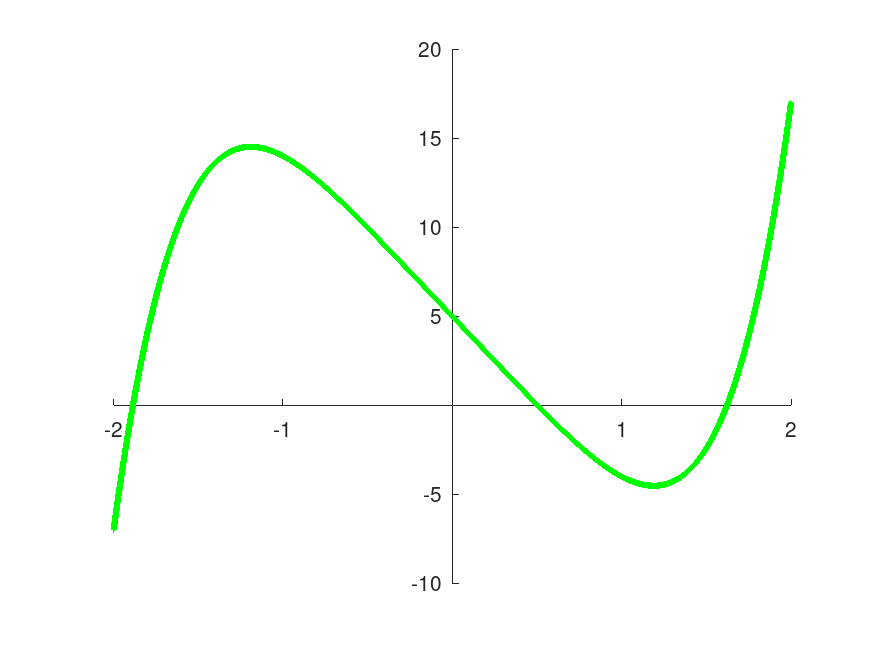
\includegraphics[width=13cm, height=7cm]{quantic2.png}
    \caption{\footnotesize Plotted by the ``GNU-Octave''}
  \end{figure}

  It has only three real roots. This polynomial is irreducible over \(\mathbb{Q}\) by the Eisenstein's criterion so by Theorem-11 its Galois group is \(S_5\) which contains \(5!=120\) elements.
 \end{example}

  \begin{tcolorbox}[colback=gray!20, colframe=blue!30, title={\small \bfseries \textcolor{black}{GNU-Octave Code for the above plotting}}, width=15cm]
\begin{boxedverbatim}
  x=-2:0.000001:2;
  y=x.^5-10*x+5;

  plot(x,y,"g","linewidth",3);
  xlabel="x";                     yabel="y";
  title="Graph of the quntic y";
  box off;
  set(gca, 'XAxisLocation', 'origin', 'YAxisLocation', 'origin');
\end{boxedverbatim}
  \end{tcolorbox}

\vspace{5mm}

\begin{example}
  The polynomial is \(f(x)=x^7-2x^5-4x^3+2x^2+4x-2\) which is irreducible over \(\mathbb{Q}\) by the Eisenstein's criterion. Its graph is shown below.

    \begin{figure}[h!]
    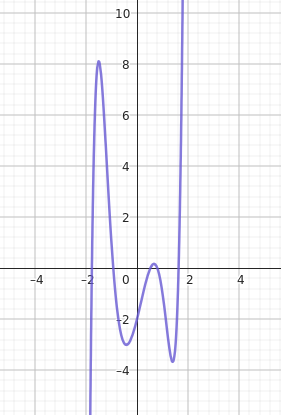
\includegraphics[width=11cm, height=7cm]{seventh2.png}
    \caption{\footnotesize Plotted by the ``Geogebra''}
  \end{figure}
The Graph shows this polynomial has exactly five real roots. So exactly two of its roots are complex. Hence by the Theorem-11 its Galois Group is \(S_7\) which contains \(7!=5040\) elements.
\end{example}

\vspace{5mm}
\section{Galois Group of Reducible polynomials}
For any polynomial \(f \in K[x]\) we factor \(f\) into irreducibles as \(f_1f_2...f_k\) and compute the Galois group \(G_i\)  of \(f_i\) for each \(i=1,2,...,k\). Then the Galois group \(G\) of \(f\) is isomorphic to a subgroup of \(\prod G_i\) \cite{algorithm}.\\

\begin{example}
  The polynomial is \(f(x) = x^4-7x^2+15\)\\
  Here, \(f(x)=(x^2-3)(x^2-5)\) so it is reducible over \(\mathbb{Q}\). Let \(f_1(x)=(x^2-3)\) and \(f_2(x)=(x^2-5)\). Then \(f_1,f_2\) are both irreducible over \(\mathbb{Q}\).\\

  The splitting field for \(f_1\) is \(\mathbb{Q}(\sqrt{3})\) so its Galois group is \({\mathbb{Z}}_2\). The splitting field for \(f_2\) is \(\mathbb{Q}(\sqrt{5})\) so its Galois group is also \({\mathbb{Z}}_2\). Now we have the Galois group of \(f\) is a subgroup of \(G={\mathbb{Z}}_2 \times {\mathbb{Z}}_2\). \\

  Since the intersection of \(\mathbb{Q}(\sqrt{3})\) and \(\mathbb{Q}(\sqrt{5})\) is trival the Galois group of \(f\) is \(G\) itself which is \textit{Klein 4-group}.
\end{example}

\begin{example}
  The polynomial is \(f(x)=x^7-5x^5-10x^3+5x^2+50x-25 \in \mathbb{Q}[x]\). This polynomial factors into irreducibles over \(\mathbb{Q}\) as \((x^2-5)(x^5-10x+5)\).\\
  The Galois group of \(x^2-5\) is \({\mathbb{Z}}_2\) and of \(x^5-10x+5\) is \(S_5\) from the example-3. Also the roots of \(x^2-5\) are \(\sqrt{5}\) and \(-\sqrt{5}\) which are not the roots of \(x^5-10x+5\) from the its graph figure-4.1, so the intersection of the splitting fields of these two factor polynomials of \(f\) is trival. Hence the Galois group of \(f\) is \(\mathbb{Z}_2 \times S_5\).
\end{example}

\vspace{7mm}
\section{Galois groups of Multi-variable Polynomials}
The Galois group of a polynomial in single variable can be generalized to the Galois group of a multi-variable polynomial.\\

\begin{example}
  The polynomial is \(f(x,y)=x+y \in \mathbb{Q}[x,y]\). Now the roots of \(f\) over all the complex numbers. Hence its Galois group is \(\mathbb{C}\).
\end{example}

\hspace{5mm}
\begin{example}
  The polynomials in \(\mathbb{Q}[x,y]\) are: \begin{align}
                         y &= x^2+1 \\
                         x+y &=1
                       \end{align}.
                       The roots of these simultaneous polynomials are \(\omega, {\omega}^2\). Then the splitting field of this system is \(\mathbb{Q}(\omega)\). Here the automorphisms of \(\mathbb{Q}(\omega)\) are: \\
       \(\omega \longmapsto \omega\) and \hspace{9mm} \(\omega \longmapsto {\omega}^2\).\\
                       Hence the Galois group of this system is \(\{(1), (1,2)\} \cong {\mathbb{Z}}_2\).
\end{example}

%%% Local Variables:
%%% mode: latex
%%% TeX-master: "n"
%%% End:




\part{Applications}
\chapter{Galois Group of a Polynomial}
Galois fields are the finite fields. They can be completely characterized in terms of splitting fields of some polynomials. It is found that the Galois group of an extension of a finite field by a finite field is shown cyclic.\\

\begin{definition}[Prime Fields]
Let \(F\) be a field and let \(P\) be the intersection of all subfields of \(F\). Then \(P\) is a field with no proper subfields. This field \(P\) is called the Prime subfield of \(F\).
\end{definition}

\begin{enumerate}
\item If \(charF=p(prime)\), then \(P\cong {\mathbb{Z}}_p\).
\item If \(charF=0\), then \(P\cong \mathbb{Q}\).
\end{enumerate}

\begin{theorem}
A  finite field \(F\) has \(p^n\) number of elements where \(p \in \mathbb{Z}_+\) is a prime and it has \(p^n\) number of elements if and only if \(F\) is a splitting field of \(x^{p^n} - x\) over \(\mathbb{Z}_p\).\\
\end{theorem}

\begin{theorem}
  If \(F\) is a finite dimensional extension field of a finite field \(K\), then \(F\) is finite and is Galois over \(K\). The Galois group \(Aut_K^F\) is cyclic.
\end{theorem}

\section{Representation of Finite Fields}
Basically there are two types of representation of a finite field. These two representations are equivalent. 
\subsection{Integer representation}

\(GF(p^n)=\{0,1,...,p-1\} \cup \{p,p+1,...,p+p-1\} \cup ... \cup \{p^{n-1},p^{n-1}+1,...,p^{n-1}+p^{n-2}+...+p-1\}\).

\begin{example}
    \(GF(2)=\{0,1\}\)\\
    \(GF(2^3)=\{0,1\} \cup \{2,2+1\} \cup \{2^2,2^2+1,2^2+2,2^2+2+1\}=\{0,1,2,3,4,5,6,7\}\)
\end{example}

But the digits \(2,3,..,7\) of the field \(GF(2^3)\) do not lie on the field \(GF(2)\). If look the field \(GF(2^3)\) as an extension field of \(GF(2)\) and write its elements only using the elements of the base field \(GF(2)\) then we have the following representations:
\vspace{3mm}

\begin{tabular}{|c|c|c|}
    \hline
    Digits & \ & Binary rep..\\
    \hline
    3 & \(2+1\) & 011 \\
    4 & \(2^2+2^1 \times 0 +2^0 \times 0\) & 100 \\
    5 & \(2^2+1\) & 110 \\
    \hline
\end{tabular}
\vspace{3mm}

This is actually \textbf{Binary representation} of the field \(GF(2^3)\)



\subsection{Polynomial representation}
For a field \(F\) and and an irreducible polynomial \(f(x) \in F[x]\) the quotient ring \(F[x]/(f(x))\) is field.\\
If \(F\) is a finite field consisting of \(p\) number of elements and \(f(x) \in F[x]\) is irreducible then \(F[x]/(f(x))\) is finite field. This field consists of all polynomials modulo \(f(x)\). If \(F=GF(2^3)\) then \(x^8+x^7+...+x+1 \in F[x]\) is irreducible in \(F[x]\). Since \(F\) has \(8\) elements which are modulo \(8\), \(F\) is represented by the factor ring \(F[x]/(f(x))\). \\


In the example above \(5\) has the representation \(2^2+1\). This gives the polynomial representation \(x^2+1=(1,0,1)\)(coefficient of \(x^2\) is \(1\) of \(x\) is \(0\) and of constant is \(1\) ) Now the binary equivalent of \(5\) is \(101\).

\section{Operations in Galois Field}
Let the Galois field be \(GF(p^n)\). Since the elements of a Galois field can be represented as polynomials the operations are similar to polynomial operations. Let \(f(x)=a_0+a_1x+..+a_{n-1}x^{n-1}\) and \(g(x)=(b_0+b_1x+...+b_{n-1}x^{n-1}\).
\begin{enumerate}
  \item Addition \\
  \(f(x)+g(x)\;\;\;\; (modp)\) 
  
  \item Multiplicaiton \\
  \(f(x).g(x)\;\;\; (modp)\)
\end{enumerate}




\end{document}
%%% Local Variables:
%%% mode: latex
%%% TeX-master: t
%%% End:
